\documentclass[12pt, a4paper, ngerman]{article}

% Metadata Setup
\newcommand{\Autor}{Paul Walker}
\newcommand{\Was}{Digitale Bildverarbeitung}
\newcommand{\Kurs}{TINF20IN}
\newcommand{\MatrikelNummer}{3610783}
\newcommand{\Studiengang}{Informatik / Informationstechnik}

\title{Wavelets; Verfahren und Einsatzgebiete}
\author{\Autor}
\date{22.03.2023}

% SETUP
\usepackage{biblatex} % für bibliografie
\usepackage{hyperref} % für links zum klicken
\usepackage{color}    % für Farben (benötigt für listings)
\usepackage{listings} % code schnipsel
\usepackage[ngerman]{babel} % lokalisierung der Titel (Inhaltsverzeichniss)
\usepackage{bookmark} % bookmarks für das PDF
\usepackage{csquotes} % korrekte quotes
\usepackage[version=3]{acro} % akronyme
\usepackage{geometry} % seitengeometrie (margin etc einstellen)
\usepackage{parskip}  % zeilenabstand bei neuem paragraph statt indentierung
\usepackage{fancyhdr} % header und footer
\usepackage{array}    % für bessere Tabellen
\usepackage{titlesec} % um die Titel anzupassen
\usepackage{plantuml} % PLANTUML_JAR has to be set and --shell-escape
\usepackage{amsfonts} % für \mathbb
\usepackage{placeins} % für \FloatBarrier
\usepackage{nicematrix}
\usepackage{tikz} 

% Tikz setup
\usetikzlibrary{positioning}

\hypersetup{
  pdfauthor={\Autor},
  pdftitle={\Was},
  hidelinks
}

\geometry{
  a4paper,
  left=25mm,
  right=25mm,
  headheight=125mm,
  top=35mm,
  bottom=30mm,
  footskip=15mm
}

% title setup 
% make paragraph have a newline
\titleformat{\paragraph}
{\normalfont\normalsize\bfseries}{\theparagraph}{1em}{}
\titlespacing*{\paragraph}
{0pt}{3.25ex plus 1ex minus .2ex}{1.5ex plus .2ex}

% add bibliography
\addbibresource{bibliography.bib}

% add Graphics
\graphicspath{ {./assets/} }

% header and footer setup
\pagestyle{fancy}
\fancyhf{}
\rhead{\Was}
\lhead{\leftmark}
\lfoot{Autor: \Autor, Kurs: \Kurs}
\rfoot{Seite \thepage}
\renewcommand{\headrulewidth}{1pt}
\renewcommand{\footrulewidth}{1pt}
\fancypagestyle{simple}{
  \fancyhf{}
  \rhead{\Was}
  \lfoot{Autor: \Autor, Kurs: \Kurs}
  \rfoot{Seite \thepage}
}

% acronyms
\acsetup{
  list/display = used,
  pages/display = first
}

%Offizele Akronyme
\DeclareAcronym{iso}{short=ISO, long=International Organization for Standardization}
\DeclareAcronym{cwt}{short=CWT, long=Stetige Wavelet Transformation}
\DeclareAcronym{dwt}{short=DWT, long=Diskrete Wavelet Transformation}
\DeclareAcronym{fwt}{short=FWT, long=Schnelle Wavelet Transformation}

\newcommand{\reals}{\ensuremath{\mathbb{R}}}
\newcommand{\natnums}{\ensuremath{\mathbb{N}}}

% code snippet setup
\renewcommand{\lstlistingname}{Code-Auszug}
\renewcommand{\lstlistlistingname}{Liste der Code-Auszüge}

\definecolor{black}{rgb}{0,0,0}
\definecolor{green}{rgb}{0,0.5,0}
\definecolor{orange}{rgb}{1,0.45,0.13}		
\definecolor{brown}{rgb}{0.69,0.31,0.31}

% python
\lstdefinelanguage{Python}{
  morekeywords={import, def, from, for, in, if, else, return, True, False, catch, return, null, switch, if, in, while, do, else, case, break},
  morecomment=[l]\#,
  morestring=[b]",
  morestring=[b]""",
  morestring=[b]'
}

\lstdefinestyle{light}{
  % General design
  basicstyle={\footnotesize\ttfamily},   
  frame=b,
  % line-numbers
  xleftmargin={0.75cm},
  numbers=left,
  stepnumber=1,
  firstnumber=1,
  numberfirstline=true,	
  % Quellcode design
  identifierstyle=\color{black},
  keywordstyle=\color{blue}\bfseries,
  ndkeywordstyle=\color{green}\bfseries,
  stringstyle=\color{orange}\ttfamily,
  commentstyle=\color{brown}\ttfamily,
  % Quellcode
  alsodigit={.:;},
  tabsize=2,
  showtabs=false,
  showspaces=false,
  showstringspaces=false,
  extendedchars=true,
  breaklines=true,
}

\begin{document}
\raggedright % sorgt dafür das alles strikt links ausgerichtet wird (und sorgt für mehr seiten)


% Titlepage
\makeatletter
\begin{titlepage}
  \begin{center}
    \vspace*{1cm}
    {\Huge\scshape \Was}\\[2cm]
    \begin{center}
      \linespread{1}\Huge \@title\\[2cm]
    \end{center}
    {\large \Studiengang}\\
    {\large Duale Hochschule Baden-Württemberg\\ Stuttgart}\\[2cm]
    {\large von}\\
    {\large\bfseries \@author}
    \vfill
  \end{center}
  \begin{tabular}{l@{\hspace{2cm}}l}
    Matrikelnummer: & \MatrikelNummer \\
    Abgabedatum:    & \@date          \\
  \end{tabular}
\end{titlepage}
\makeatother

% Table of content
\tableofcontents
\newpage

\thispagestyle{simple}
\printacronyms[name=Abkürzungsverzeichnis, heading=section*]
\newpage

%%%%%%
% Content here
%%%%%% 

\renewcommand{\abstractname}{Abstract} % dass Abstract auch Abstract heißt und nicht zusammenfassung
\begin{abstract}
  Abstract Stuff
\end{abstract}

\section{Einleitung}

Wavelets spielen in der heutigen Bildverarbeitung eine große Rolle.
Sie erlauben es Signale zu analysieren, Signale zu komprimieren,
Rauschen zu entfernen und vieles mehr.
Die Wavelet Transformation hat einige Ähnlichkeiten mit der Fourier Transformation
allerdings ist die Wavelet Transformation in der Lage Signale
auch in der Zeitdomäne zu analysieren~\cite{wavelets_intro}.
Im Gegensatz zur Fourier Transformation lassen sich mit der Wavelet Transformation
speziell Lokale Effekte in einem Signal analysieren,
diese Eigenschaft ist besonders nützlich bei der Analyse von Bildern und Audio Signalen
und kann unter anderem auch für die Komprimierung dieser Daten eingesetzt werden.
Wavelets könnten so beispielsweise genutzt werden,
um die Frequenz von einer Musikaufnahme zu analysieren.
Die Wavelet Transformation ermöglicht es dabei die Frequenzen der Töne zu bestimmen
und zu bestimmen, wann und wie lange diese Töne gespielt werden~\cite[S.17]{wavelet_patterns}.
Es lässt sich in diesem Beispiel also die musikalische Notation
eines Stückes rekonstruieren.

\section{Verfahren}
\label{sec:verfahren}

Der Begriff Wavelet kommt von dem Begriff \emph{Wave} also Welle
und \emph{let} als Verkleinerungsform, also kleine Welle~\cite[S.2]{wavelet_patterns}.
Für die Wavelet Transformation wird zuerst eine Basisfunktion gewählt,
das sogenannte \emph{Analyse Wavelet} oder \emph{Mutter Wavelet}~\cite{wavelets_intro}.
Mit dieser Basisfunktion wird dann das Signal analysiert.
Die Basisfunktion wird dabei mit \(\Psi(t)\) bezeichnet.
Für die Wavelet Transformation wird die Basisfunktion skaliert und verschoben.

Es können verschiedene Arten von Basisfunktionen gewählt werden,
einige davon werden in Abschnitt~\ref{sec:basis_functions} vorgestellt.
Alle Basisfunktionen müssen jedoch einige Eigenschaften erfüllen.
Eine wichtige Eigenschaft ist die sogenannte \emph{admisibility} Bedingung~\cite[S.6]{friendly_wavelet}.
Diese sagt aus, dass die Basisfunktion eine oszillierende Funktion sein muss,
deren Integral über die Zeit null sein muss~\cite[S.6]{friendly_wavelet}.
Eine weitere wichtige Eigenschaft ist die \emph{Regularität} des Wavelets.
Die sorgt für einen schnellen Zerfall des Wavelets,
also dafür das die Basisfunktion schnell gegen null geht~\cite[S.6]{friendly_wavelet}.
Die genannten Eigenschaften reichen nicht aus um ein Wavelet zu definieren,
geben aber Aufschluss über die Form einer Wavelet Funktion
als schwingende und schnell abfallende Funktion.
Es wird kein spezielles Wavelet vorgegeben,
viel ist es möglich mit diesen Rahmenbedingungen Basisfunktionen zu wählen,
die für die jeweiligen Anwendungsfälle angepasst sind~\cite[S.5]{friendly_wavelet}.

\subsection{\acl{cwt}}

Für die \ac{cwt} wird das Mutter Wavelet skaliert und verschoben.
Der Skalierungsfaktor wird mit \(s\) bezeichnet
und die Verschiebung des Wavelets mit \(\tau\).
Das geschieht mit der folgenden Formel.
Dabei dient \(\frac{1}{\sqrt{s}}\) zur Normalisierung der Funktion~\cite[S.5]{friendly_wavelet}.

\[
  \Psi_{s,\tau}(t)=\frac{1}{\sqrt{s}}\Psi(\frac{t-\tau}{s})
\]

Das skalierte und verschobene Wavelet wird dann mit dem Signal multipliziert.
Über das Ergebnis wird dann integriert.
Es ergibt sich die folgende Wavelet Transformation \(W(s,\tau)\)~\cite[S.5]{friendly_wavelet}

\[
  W(s,\tau)=\int_{-\infty}^{\infty}f(t)\Psi_{s,\tau}(t)dt
\]

Damit ergibt sich eine zweidimensionale Funktion.
Die Dimension \(\tau\) beschreibt dabei den Zeitbereich des Signals
und die Dimension \(s\) beschreibt den Frequenzbereich des Signals.
Wenn die Wavelet Transformation auf einem zweidimensionalen Signal ausgeführt wird,
dann ergibt sich eine vierdimensionale Wavelet Transformation~\cite[S.6]{friendly_wavelet}.
Die Rücktransformation der Wavelet Transformation sieht wie folgt aus~\cite[S.5]{friendly_wavelet}

\[
  f(t)=\int_{-\infty}^{\infty}\int_{-\infty}^{\infty}W(s,\tau)\Psi_{s,\tau}(t)dsd\tau
\]

\subsection{\acl{dwt}}

Die \ac{cwt} wandelt ein eindimensionales Signal
in einen zweidimensionalen Bereich.
Das stellt allerdings eine Große Redundanz dar.
Eine Lösung dafür ist es Wavelets nicht kontinuierlich
zu skalieren und zu verschieben, sondern beide Werte zu diskretisieren~\cite[S.8]{friendly_wavelet}.

\[
  \Psi_{j,k}=\frac{1}{\sqrt{s_0^j}}\Psi(\frac{t-k\tau_0s_0^j}{s_0^j})\;;j\in\mathbb{Z},k\in\mathbb{Z},s_0>1
\]

Mit diesen diskreten Wavelet Koeffizienten lässt sich nun ein Signal analysieren.
Das Mutter Wavelet und damit die Transformation ist allerdings weiterhin stetig~\cite[S.8]{friendly_wavelet}.
Die Transformation kann diskretisiert werden,
indem die Wavelet Funktion diskretisiert wird.
Allerdings kann eine höhere Auflösung erzielt werden,
wenn die Wavelet Transformation in zwei Teile,
einen Höherfrequenten Teil und einen Niedrigfrequenten Teil
aufgespalten wird~\cite[S.14]{friendly_wavelet}.

\[
  \begin{array}{c}
    W_\varphi(j,k) = \frac{1}{\sqrt{M}}\sum_{x=0}^{M-1}f(x)\varphi_{j,k}(x) \\
    W_\Psi(j,k) = \frac{1}{\sqrt{M}}\sum_{x=0}^{M-1}f(x)\Psi_{j,k}(x)
  \end{array}
\]

Dabei beschreibt \(j\) die Skalierung des Wavelets
und \(k\) die Verschiebung~\cite[S.9]{wavelet_analysis}.

\subsection{\acl{fwt}}

Die \ac{fwt} ist eine Weiterentwicklung der \ac{dwt},
die es möglich macht die \ac{dwt} effizienter auszuführen.
Dafür wird die Trennung der \ac{dwt} in Höherfrequenten
und Niedrigfrequenten Teil ausgenutzt.
Eine Wavelet Transformation lässt sich basierend
auf der Nächsten Wavelet Transformation ausdrücken.
Wenn für \(\varphi(x)\) und analog für \(\Psi(x)\) gilt

\[
  \varphi(x) = \sum_n h_{\varphi}(n)\sqrt{2}\varphi(2x-n)
\]

Dann ergibt sich für \(W_\varphi(j,k)\) die folgende Gleichung~\cite[S.11]{wavelet_analysis}.

\[
  W_\varphi(j,k)=\sum_m h_\varphi(m-2k)W_\varphi(j-1,m)
\]

Und analog dazu für \(W_\Psi(j,k)\)~\cite[S.11]{wavelet_analysis}.

\[
  W_\Psi(j,k)=\sum_m h_\Psi(m-2k)W_\Psi(j-1,m)
\]

Damit lässt sich die Wavelet Transformation für ein bestimmtes \(j\)
einfach aus dem vorherigen \(j\) bilden.
Es entsteht ein Berechnungsbaum mit dem die Wavelet Transformation
einfach und schnell berechnet werden kann.
Dieser Berechnungsbaum ist in Abbildung~\ref{fig:wavelet_tree} dargestellt.
Um eine Stufe der \ac{fwt} zu berechnen,
muss die Funktion \(h_\Psi(-n)\) und \(h_\varphi(-n)\) mit \(n=2k,k\leq 0\)
auf die vorherige Stufe der Wavelet Transformation angewendet werden.
Nach einem Subsampling mit dem Faktor 2 erhält man
die nächste Stufe der Wavelet Transformation~\cite[S.12]{wavelet_analysis}.
Um weitere Frequenzstufen zu erhalten,
wird der Berechnungsbaum um weitere Stufen vergrößert.

\begin{figure}
  \centering
  \begin{tikzpicture}[
      squarednode/.style={rectangle, draw=black, thick, minimum size=5mm},
    ]
    \node (start) {\(W_\varphi(j+1,n)\)};
    \node[squarednode] (down1) [above right=of start] {\(h_\Psi(-n)\)};
    \node[squarednode] (sub1) [right=of down1] {\(2\downarrow\)};
    \node (w1) [right=of sub1] {\(W_\Psi(j,n)\)};
    \node[squarednode] (down2) [below right=of start] {\(h_\varphi(-n)\)};
    \node[squarednode] (sub2) [right=of down2] {\(2\downarrow\)};
    \node (w2) [right=of sub2] {\(W_\varphi(j,n)\)};
    \draw[thick,->] (start.north) -- (down1.west);
    \draw[thick,->] (down1.east) -- (sub1.west);
    \draw[thick,->] (sub1.east) -- (w1.west);
    \draw[thick,->] (start.south) -- (down2.west);
    \draw[thick,->] (down2.east) -- (sub2.west);
    \draw[thick,->] (sub2.east) -- (w2.west);
  \end{tikzpicture}
  \caption{Wavelet Berechnungsbaum}
  \label{fig:wavelet_tree}
\end{figure}

\subsection{Basis Funktionen}
\label{sec:basis_functions}
% Was gibt es für verschiedene Basis funktionen,
% wofür sind die jeweils nützlich

In der Wavelet Transformation können verschiedene Basisfunkionen verwendet werden,
allerdings müssen alle Basisfunktionen gewisse Eigenschaften erfüllen,
diese wurden bereits in Abschnitt~\ref{sec:verfahren} beschrieben.
Solange diese Eigenschaften beachtet werden,
können Wavelets an verschiedene Anwendungsfälle angepasst werden.
Zur Erkennung von bestimmten Mustern auf einem Bild
werden sicherlich andere Basisfunktionen verwendet als zum Entrauschen eines Bildes.
In Abbildung~\ref{fig:basis_functions} sind einige mögliche Wavelet Basisfunktionen dargestellt.
Dabei sind sowohl das Haar als auch das Daubechies Wavelet Beispiele für diskrete Wavelets
und das Mexican Hat und das Morlet Wavelet Beispiele für kontinuierliche Wavelets.

\begin{figure}
  \centering
  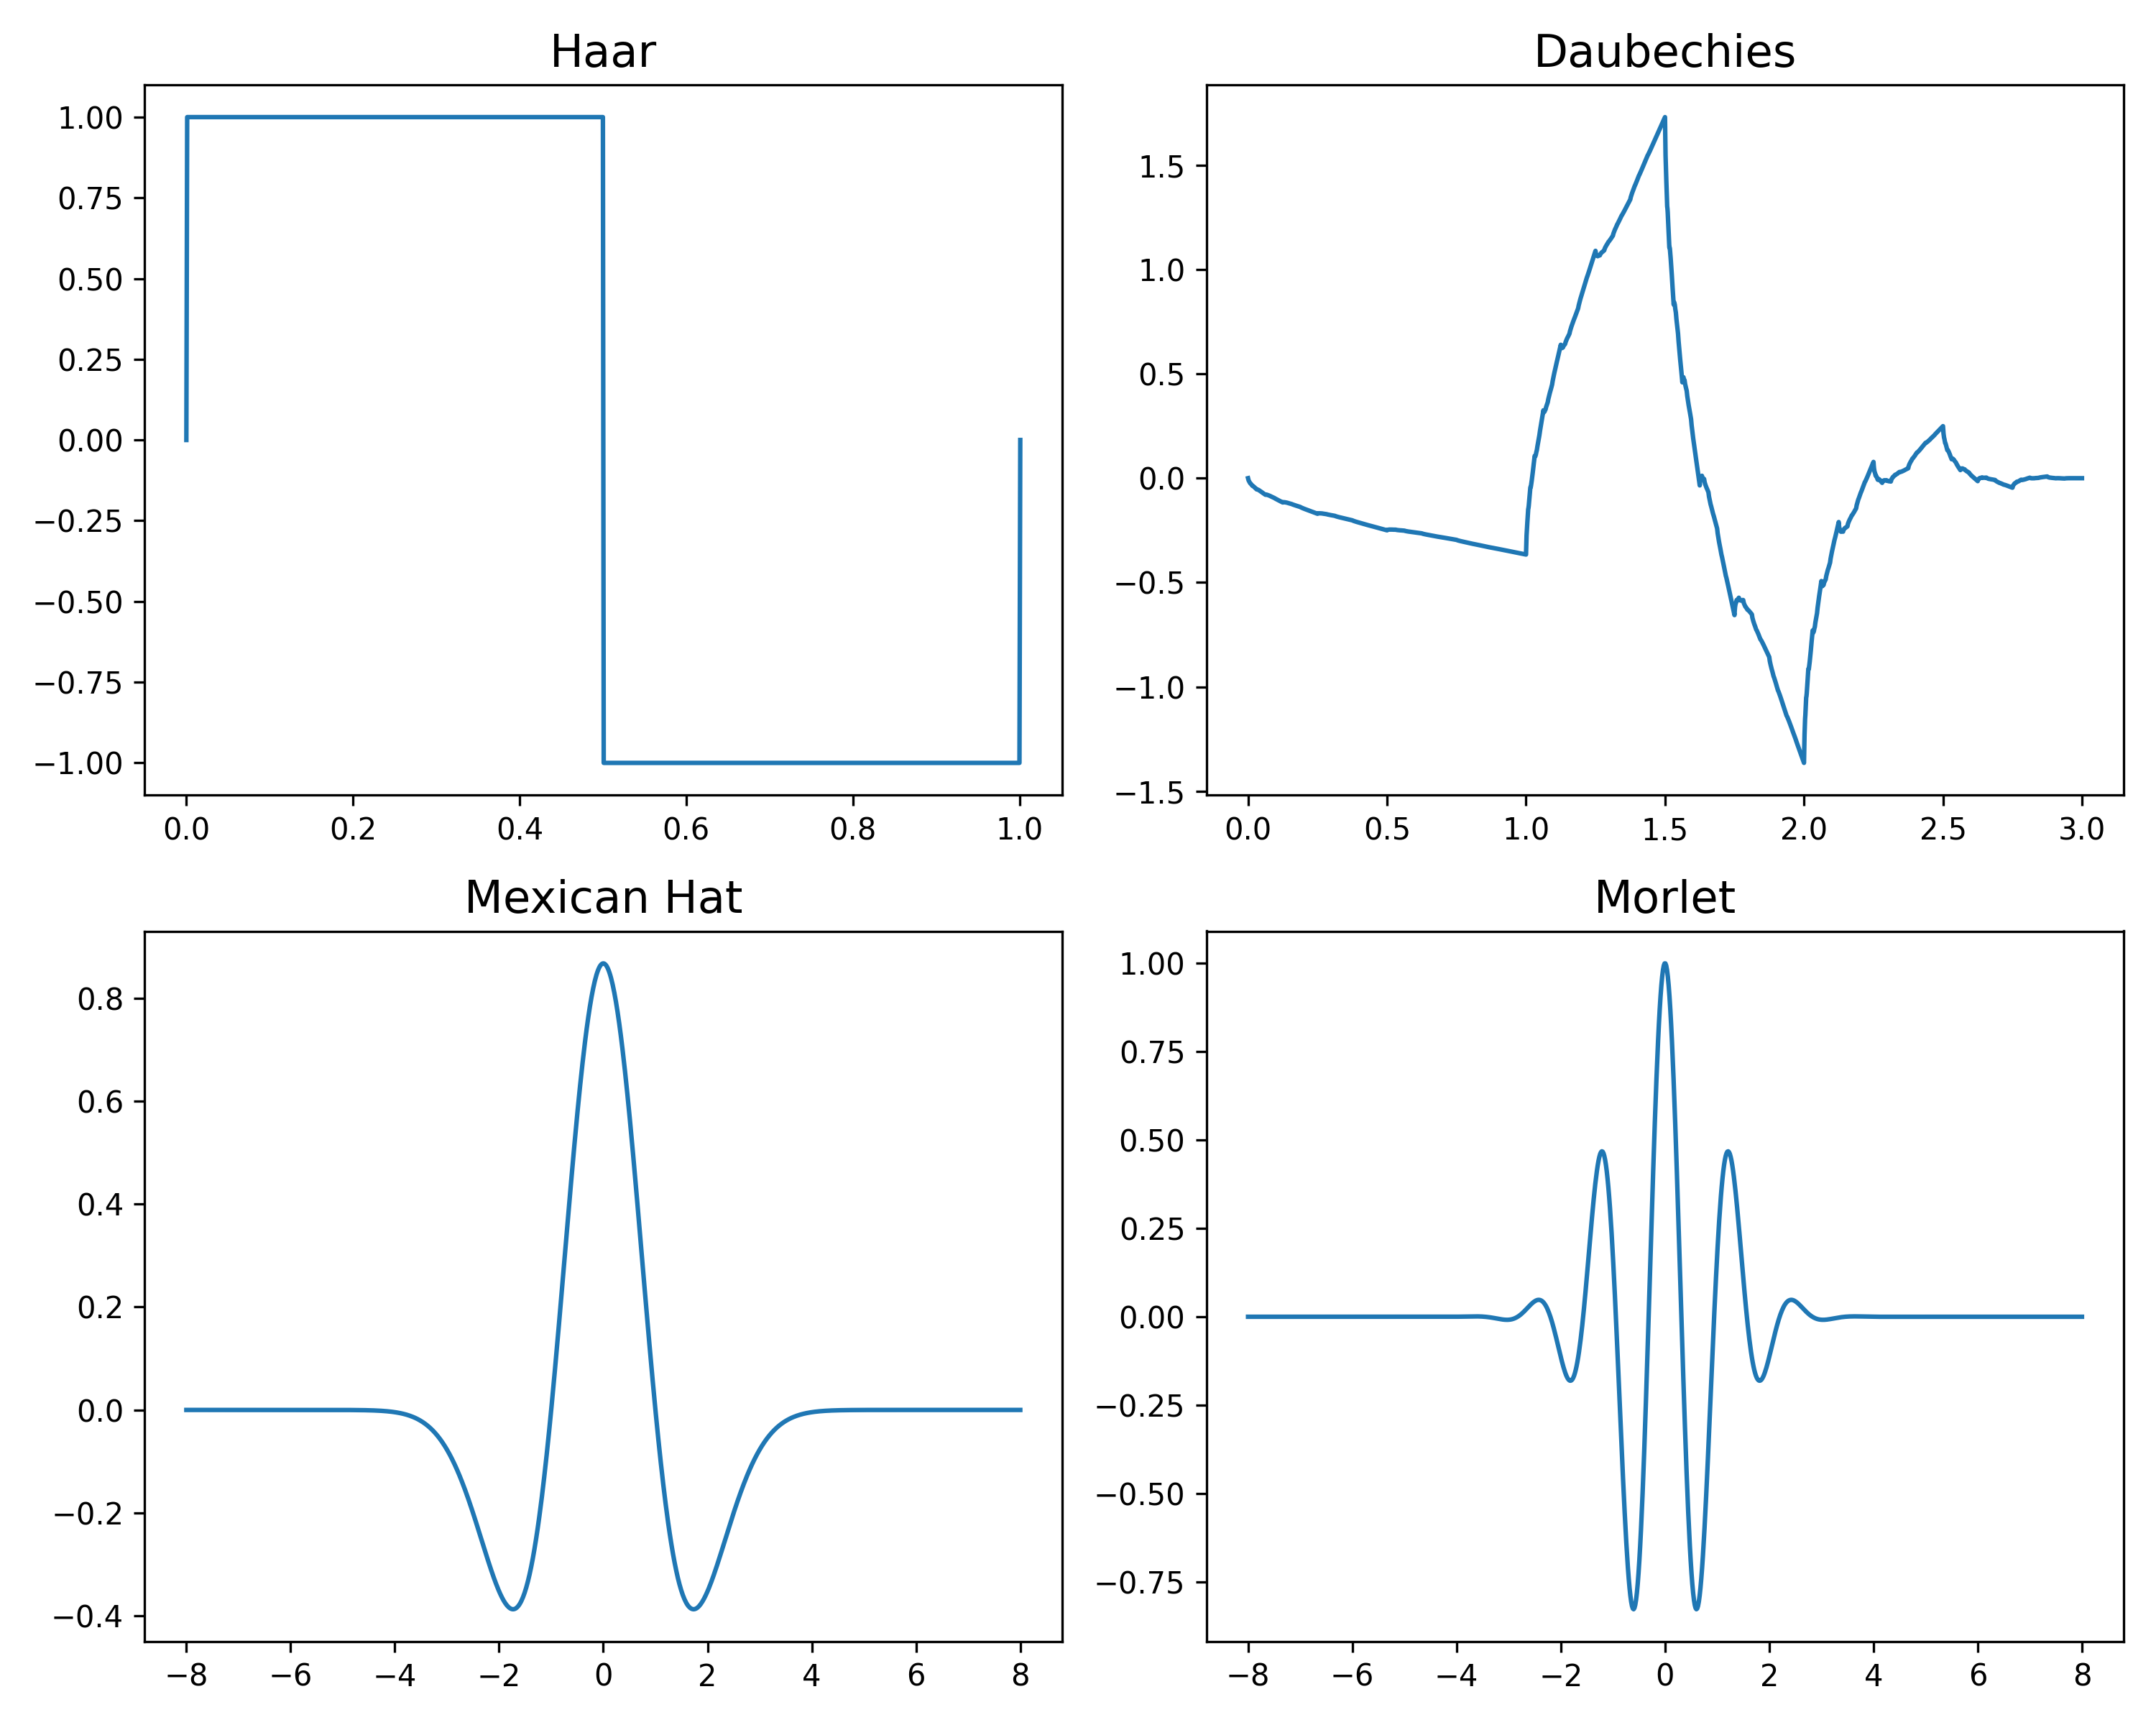
\includegraphics[width=\textwidth]{wavelets.png}
  \caption{Basisfunktionen}
  \label{fig:basis_functions}
\end{figure}

\section{Wavelet versus Fourier}

Die Wavelet Transformation hat einige Ähnlichkeiten zur Fourier Transformation.
Es wird in beiden fällen die Zusammensetzung des Signals aus Basisfunktionen bestimmter Frequenzen analysiert.
Bei der Fourier Transformation ist die Basisfunktion eine Sinus oder Cosinus Funktionen~\cite[S.5]{wavelets_intro}.
Die Wavelet Transformation schränkt die Basisfunktion nicht auf Sinus oder Cosinus Funktionen ein.
Hier sind alle Funktionen erlaubt, die nicht unendlich sind und ein Integral von 1 haben.
Die Fourier Transformation ist nur in der Lage den Frequenzbereich eines Signals zu analysieren.
Die Wavelet Transformation macht es dagegen möglich den Frequenzbereich und den Zeitbereich eines Signals
gleichzeitig zu analysieren und so Zusammenhänge zwischen den beiden Bereichen zu erkennen,
um so weitere Aufschlüsse über das Signal zu erhalten.
Außerdem können bei der Wavelet Transformation verschiedene Basisfunktionen genutzt werden,
das macht es möglich die Basisfunktionen an den Anwendungsfall anzupassen.
Die Fourier Transformation ist dagegen auf die Sinus und Cosinus Funktionen beschränkt.

\section{Einsatzgebiete}

Wavelets werden in vielen Bereichen eingesetzt,
vor allem in Bereichen, die mit digitaler Signalverarbeitung zu tun haben.
Typische Anwendungen finden sich in der Bildverarbeitung, der Bildkompression und der Audioanalyse,
aber auch in vielen anderen Bereichen wird die Wavelet Transformation eingesetzt.
Hier sollen allerdings nur einige wenige Anwendungen vorgestellt werden.

\subsection{Bildverarbeitung}

% TODO grafik hier.

In der Bildverarbeitung wird in der Regel eine zweidimensionale Wavelet Transformation verwendet,
um ein Bild zu analysieren.
Mithilfe der Wavelet Transformation kann ein Bild in verschiedene Frequenzbereiche zerlegt werden,
so können Aktionen nur auf bestimmten Frequenzbereichen durchgeführt werden~\cite[S.38]{dt_manual}.
In Abbildung~\ref{TODO} ist ein Bild und einige seiner Frequenzbereiche dargestellt.
Es ist erkennbar, dass die verschiedenen Frequenzbereiche unterschiedliche Details enthalten.
% TODO Bild beschreiben.
Mit der Zerlegung des Bildes in einzelne Frequenzbereiche über die Wavelet Transformation
lassen sich einige Aufgaben in der Bildverarbeitung vereinfachen.
Hier werden ein paar Beispiele für die Anwendung von Wavelets in der Bildverarbeitung gezeigt.

\subsubsection{Entrauschen}

Typischerweise ist das Rauschen eines Kamerasensors
hauptsächlich in den höheren Frequenzbereichen des Bildes zu erkennen.
Diese Frequenzbereiche lassen sich dann mit der Wavelet Transformation isolieren.
Dann können die Frequenzbereiche, in denen sich das Rauschen befindet,
getrennt von allen anderen Frequenzbereichen bearbeitet werden,
um das Rauschen zu reduzieren~\cite[S.117]{dt_manual}.
Das Rauschen wird dann allerdings von einem anderen Filter
der nicht teil der Wavelet Transformation ist entfernt.
Das Rauschen in einem Bild kann über verschiedene Frequenzbereiche verteilt
und in verschiedenen Frequenzbereichen verschieden stark sein~\cite[S.119]{dt_manual}.
Die Aufspaltung des Bildes in verschiedene Frequenzbereiche
macht es möglich in den einzelnen Frequenzbereichen
das Rauschen unterschiedlich stark zu reduzieren~\cite[S.119]{dt_manual}.
So kann pro Frequenzbereich ein Kompromiss zwischen der Reduktion des Rauschens
und dem Erhalten von Details im Bild gefunden werden.

\subsubsection{Retuschieren}
\subsubsection{Lokaler Kontrast}
\subsection{Bildkompression}
\subsection{Audioanalyse}

\newpage
\printbibliography

\end{document}
